\documentclass{prova}

\usepackage{amsmath}
\usepackage{amsfonts}

\setlength{\textheight}{25cm}

\renewcommand{\sin}{\,\mbox{sen}\,}
\newcommand{\tg}{\,\mbox{tg}\,}
\newcommand{\ds}{\displaystyle}

\professor{Prof.\@ Adriano Barbosa}
\disciplina{C\'alculo Diferencial e Integral}
\avaliacao{PS}
\curso{Engenharia de Aquicultura}
\data{29/11/2021}

\begin{document}
	\cabecalho{5}  % o numero 5 indica a qnt de quadros na tabela de nota

    \textbf{Todas as respostas devem ser justificadas.}

    \vspace{0.5cm}
    \textbf{Avalia\c{c}\~ao P1:}
    \begin{questionario}
        \q{Calcule os limites a seguir:}
            \begin{questionario}
                \qq{$\ds\lim_{t\rightarrow 4} \frac{\sqrt{x}-2}{x^2-4x}$}
                \qq{$\ds\lim_{x\rightarrow -3} f(x)$, onde
                $f(x)=\left\{
                    \begin{array}{rl}
                        \ds\frac{x^2+x-6}{x+3}, & \mbox{ se } x<-3 \\
                        & \\
                        \ds\cos\left(\frac{\pi x}{3}\right), & \mbox{ se } x \geq -3
                    \end{array}
                \right.$}
            \end{questionario}
        \q{Se $-2x+6 \leq f(x) \leq x^2-4x+7$, encontre
        $\ds\lim_{x\rightarrow 1} f(x)$.}
        \q{Suponha que a fun\c{c}\~ao $f$ \'e cont\'{\i}nua para todo $x\in\mathbb{R}$ e
        que $f(-2)=3$, $f(-1)=-1$, $f(0)=-4$, $f(1)=1$ e $f(2)=5$. Em quais
        dos intervalos abaixo o Teorema do Valor Intermedi\'ario garante que
        $f(x)=0$ possui uma raiz real?}
            \begin{questionario}
                \qq{$[-2,1]$}
                \qq{$[-1,0]$}
                \qq{$[-1,1]$}
                \qq{$[0,2]$}
            \end{questionario}
        \q{Calcule a segunda derivada da fun\c{c}\~ao $f(x) = \cos(x)\sin(x)$.}
        \q{Se uma pedra for lan\c{c}ada para cima no planeta Marte com
        velocidade de $16m/s$, sua altura (em metros) ap\'os $t$ segundos \'e
        dada por $H(t)=16t-1,6t^2$.}
            \begin{questionario}
                \qq{Encontre a velocidade da pedra como uma fun\c{c}\~ao de $t$.
                Qual a velocidade ap\'os 3 segundos?}
                \qq{Encontre a acelera\c{c}\~ao da pedra como uma fun\c{c}\~ao de $t$.
                Qual a acelera\c{c}\~ao ap\'os 3 segundos?}
                \qq{D\^e uma equa\c{c}\~ao da reta tangente ao gr\'afico de $H(t)$ no
                ponto $(3, 33.6)$.}
            \end{questionario}
    \end{questionario}

    \vspace{0.5cm}
    \textbf{Avalia\c{c}\~ao P2:}
    \begin{questionario}
        \q{\hfill{}}
            \begin{questionario}
                \qq{Se o gr\'afico da derivada de $f$ \'e o dado abaixo, determine
                os intervalos de crescimento e decrescimento de $f$ e
                classifique seus pontos cr\'{\i}ticos em m\'aximo ou m\'{\i}nimo no
                intervalo $(0,9)$.}
                \begin{figure}[h]
                    \centering
                    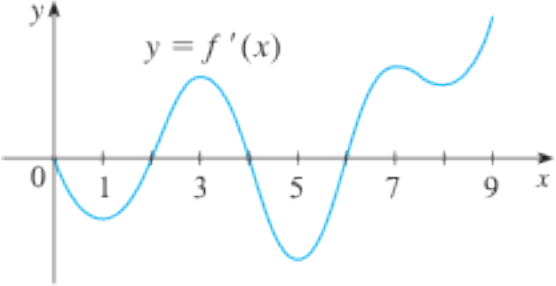
\includegraphics[width=0.3\textwidth]{q1a.png}
                \end{figure}
                \qq{Se o gr\'afico da segunda derivada de $f$ \'e o dado abaixo,
                determine os intervalos de concavidade e as coordenadas $x$ dos
                pontos de inflex\~ao no intervalo $(0,8)$.}
                \begin{figure}[h]
                    \centering
                    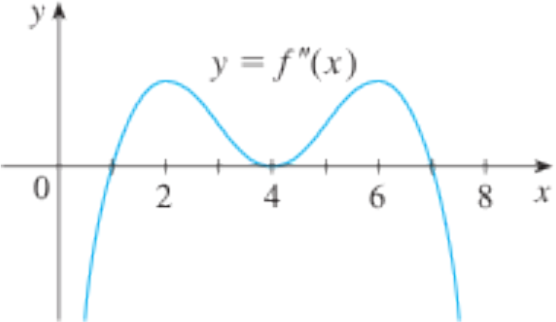
\includegraphics[width=0.3\textwidth]{q1b.png}
                \end{figure}
            \end{questionario}
        \q{Uma mosca percorre um caminho determinado pelas equa\c{c}\~oes}
            \[x(t) = \frac{1}{4} + \frac{e^{2t}}{2} - e^t,\ y(t) =
            \frac{2t}{t^2+2},\ 0\leq t\leq \ln{4}\]
            \begin{figure}[h]
                \centering
                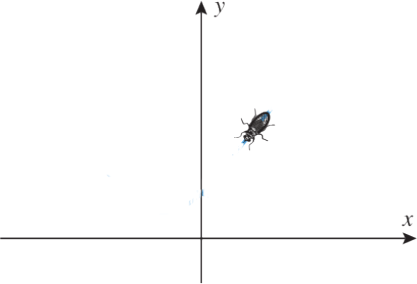
\includegraphics[width=0.3\textwidth]{q2.png}
            \end{figure}
            onde $x$ descreve o movimento horizontal e $y$ o movimento vertial da mosca.
            \begin{questionario}
                \qq{Qual a dist\^ancia mais \`a esquerda da origem que a mosca voa
                (que ocorre no menor valor de $x$)? E qual \`a direita (que
                ocorre no maior valor de $x$)?}
                \qq{Qu\~ao alto e qu\~ao baixo a mosca voa (maior e menor valor de $y$)?}
            \end{questionario}
        \q{Ao meio dia, o navio $A$ est\'a $150km$ a leste do navio $B$. O navio
        $A$ est\'a navegando para oeste a $35km/h$ e o navio $B$ est\'a navegando
        para norte a $25km/h$. Qu\~ao r\'apido varia a dist\^ancia entre os navios \`as
        16 horas? Ela est\'a aumentando ou diminuindo nesse hor\'ario?}
        \pagebreak
        \q{Uma part\'{\i}cula move-se ao longo de um eixo e sua velocidade no
        instante $t$ \'e dada pela fun\c{c}\~ao}
            \[v(t) = \int_0^t e^{x^2}\ dx.\]
            \begin{questionario}
                \qq{Encontre a fun\c{c}\~ao $a(t)$ que d\'a a acelera\c{c}\~ao da part\'{\i}cula
                no instante $t$.}
                \qq{Encontre a velocidade e a acelera\c{c}\~ao iniciais.}
            \end{questionario}
        \q{O c\'alculo da integral abaixo est\'a correto? Justifique sua resposta.}
            \[\int_{-1}^1 \frac{1}{x^2}\ dx = \int_{-1}^1 x^{-2}\ dx =
            \left.\frac{x^{-1}}{-1}\right|_{-1}^1 =
            \left.-\frac{1}{x}\right|_{-1}^1 = -1+1 = 0\]
    \end{questionario}
\end{document}
